\documentclass[a4paper,10pt,twoside,hyperpdf,fleqn]{hepthesis}

\usepackage{listings}
\usepackage{microtype}
%\usepackage[fleqn]{amsmath}
\usepackage[absolute]{textpos}
\usepackage{xspace}
\usepackage{morefloats,subfig,afterpage}
\usepackage{mathrsfs} % script font
\usepackage{verbatim}
%\usepackage[prependcaption,textsize=small]{todonotes}
\usepackage{xcolor}
\usepackage{float}
\usepackage{pifont}
\usepackage[percent]{overpic}
\usepackage{commath}
\usepackage{multirow}
\usepackage[section]{placeins}
\usepackage{amssymb}
\usepackage[Bjornstrup]{fncychap}
\usepackage{esint}
%\usepackage{lineno}
\usepackage{nicefrac}
\usepackage[super]{nth}
\usepackage{needspace}

%\input{figures/latex/tikz_includes}
% taken from
% http://www.lns.cornell.edu/~pt267/files/code/TikZFeynman.tex

\usepackage{tikz}
\usetikzlibrary{arrows,shapes}
\usetikzlibrary{trees}
\usetikzlibrary{matrix,arrows} 				% For commutative diagram
											% http://www.felixl.de/commu.pdf
\usetikzlibrary{positioning}				% For "above of=" commands
\usetikzlibrary{calc,through}				% For coordinates
\usetikzlibrary{decorations.pathreplacing}  % For curly braces
% http://www.math.ucla.edu/~getreuer/tikz.html
\usepackage{pgffor}							% For repeating patterns

\usetikzlibrary{decorations.pathmorphing}	% For Feynman Diagrams
\usetikzlibrary{decorations.markings}
\tikzset{
	>=stealth', %%  Uncomment for more conventional arrows
    vector/.style={decorate, decoration={snake}, draw},
	provector/.style={decorate, decoration={snake,amplitude=2.5pt}, draw},
	antivector/.style={decorate, decoration={snake,amplitude=-2.5pt}, draw},
    fermion/.style={draw=black, postaction={decorate},
        decoration={markings,mark=at position .55 with {\arrow{>}}}},
    fermionbar/.style={draw=black, postaction={decorate},
        decoration={markings,mark=at position .55 with {\arrow{<}}}},
    fermionnoarrow/.style={draw=black},
    gluon/.style={decorate, draw=black,
        decoration={coil,amplitude=4pt, segment length=5pt}},
    scalar/.style={dashed,draw=black, postaction={decorate},
        decoration={markings,mark=at position .55 with {\arrow{>}}}},
    scalarbar/.style={dashed,draw=black, postaction={decorate},
        decoration={markings,mark=at position .55 with {\arrow{<}}}},
    scalarnoarrow/.style={dashed,draw=black},
    electron/.style={draw=black, postaction={decorate},
        decoration={markings,mark=at position .55 with {\arrow{>}}}},
	bigvector/.style={decorate, decoration={snake,amplitude=4pt}, draw},
}

%% Using Babel allows other languages to be used and mixed-in easily
%\usepackage[ngerman,english]{babel}
\usepackage[english]{babel}
\selectlanguage{english}

%% Citation system tweaks
\usepackage{cite}
% \let\@OldCite\cite
% \renewcommand{\cite}[1]{\mbox{\!\!\!\@OldCite{#1}}}

\definecolor{color0}{RGB}{0,0,0} % Black
\definecolor{color1}{RGB}{0,83,159} % RWTH blue
\definecolor{color2}{RGB}{227,0,102} % RWTH magenta

%% Maths
% TODO: rework or eliminate maybemath
\usepackage{latex/abmath}
\DeclareRobustCommand{\mymath}[1]{\ensuremath{\maybebmsf{#1}}}
% \DeclareRobustCommand{\parenths}[1]{\mymath{\left({#1}\right)}\xspace}
% \DeclareRobustCommand{\braces}[1]{\mymath{\left\{{#1}\right\}}\xspace}
% \DeclareRobustCommand{\angles}[1]{\mymath{\left\langle{#1}\right\rangle}\xspace}
% \DeclareRobustCommand{\sqbracs}[1]{\mymath{\left[{#1}\right]}\xspace}
% \DeclareRobustCommand{\mods}[1]{\mymath{\left\lvert{#1}\right\rvert}\xspace}
% \DeclareRobustCommand{\modsq}[1]{\mymath{\mods{#1}^2}\xspace}
% \DeclareRobustCommand{\dblmods}[1]{\mymath{\left\lVert{#1}\right\rVert}\xspace}
% \DeclareRobustCommand{\expOf}[1]{\mymath{\exp{\!\parenths{#1}}}\xspace}
% \DeclareRobustCommand{\eexp}[1]{\mymath{e^{#1}}\xspace}
% \DeclareRobustCommand{\plusquad}{\mymath{\oplus}\xspace}
% \DeclareRobustCommand{\logOf}[1]{\mymath{\log\!\parenths{#1}}\xspace}
% \DeclareRobustCommand{\lnOf}[1]{\mymath{\ln\!\parenths{#1}}\xspace}
% \DeclareRobustCommand{\ofOrder}[1]{\mymath{\mathcal{O}\parenths{#1}}\xspace}
% \DeclareRobustCommand{\SOgroup}[1]{\mymath{\mathup{SO}\parenths{#1}}\xspace}
% \DeclareRobustCommand{\SUgroup}[1]{\mymath{\mathup{SU}\parenths{#1}}\xspace}
% \DeclareRobustCommand{\Ugroup}[1]{\mymath{\mathup{U}\parenths{#1}}\xspace}
% \DeclareRobustCommand{\I}[1]{\mymath{\mathrm{i}}\xspace}
% \DeclareRobustCommand{\colvector}[1]{\mymath{\begin{pmatrix}#1\end{pmatrix}}\xspace}
\DeclareRobustCommand{\Rate}{\mymath{\Gamma}\xspace}
\DeclareRobustCommand{\RateOf}[1]{\mymath{\Gamma}\parenths{#1}\xspace}

%% High-energy physics stuff
\usepackage{latex/abhep}
\usepackage{hepnames}
\usepackage{hepunits}

\makeatletter
\newcommand\footnoteref[1]{\protected@xdef\@thefnmark{\ref{#1}}\@footnotemark}
\makeatother

% Some software programs (alphabetized)
% from cms-tdr/utils/trunk/general/ptdr-definitions.sty
\newcommand{\ACERMC} {\textsc{AcerMC}\xspace}
\newcommand{\ALPGEN} {{\textsc{alpgen}}\xspace}
\newcommand{\CALCHEP} {{\textsc{CalcHEP}}\xspace}
\newcommand{\CHARYBDIS} {{\textsc{charybdis}}\xspace}
\newcommand{\CMKIN} {\textsc{cmkin}\xspace}
\newcommand{\CMSIM} {{\textsc{cmsim}}\xspace}
\newcommand{\CMSSW} {{\textsc{CMSSW}}\xspace}
\newcommand{\COBRA} {{\textsc{cobra}}\xspace}
\newcommand{\COCOA} {{\textsc{cocoa}}\xspace}
\newcommand{\COMPHEP} {\textsc{CompHEP}\xspace}
\newcommand{\EVTGEN} {{\textsc{evtgen}}\xspace}
\newcommand{\FAMOS} {{\textsc{famos}}\xspace}
\newcommand{\FEWZ} {{\textsc{fewz}}\xspace}
\newcommand{\GARCON} {\textsc{garcon}\xspace}
\newcommand{\GARFIELD} {{\textsc{garfield}}\xspace}
\newcommand{\GEANE} {{\textsc{geane}}\xspace}
\newcommand{\GEANTfour} {{\textsc{Geant~4}}\xspace}
\newcommand{\GEANTthree} {{\textsc{Geant~3}}\xspace}
\newcommand{\GEANT} {{\textsc{Geant}}\xspace}
\newcommand{\HDECAY} {\textsc{hdecay}\xspace}
\newcommand{\HERWIG} {{\textsc{herwig}}\xspace}
\newcommand{\HERWIGpp} {{\textsc{herwig++}}\xspace}
\newcommand{\HIGLU} {{\textsc{higlu}}\xspace}
\newcommand{\HIJING} {{\textsc{hijing}}\xspace}
\newcommand{\IGUANA} {\textsc{iguana}\xspace}
\newcommand{\ISAJET} {{\textsc{isajet}}\xspace}
\newcommand{\ISAPYTHIA} {{\textsc{isapythia}}\xspace}
\newcommand{\ISASUGRA} {{\textsc{isasugra}}\xspace}
\newcommand{\ISASUSY} {{\textsc{isasusy}}\xspace}
\newcommand{\ISAWIG} {{\textsc{isawig}}\xspace}
\newcommand{\MADGRAPH} {\textsc{MadGraph}\xspace}
\newcommand{\MCATNLO} {MC@NLO\xspace}
\newcommand{\AMCATNLO} {aMC@NLO\xspace}
\newcommand{\MCFM} {\textsc{mcfm}\xspace}
\newcommand{\MILLEPEDE} {{\textsc{millepede}}\xspace}
\newcommand{\ORCA} {{\textsc{orca}}\xspace}
\newcommand{\OSCAR} {{\textsc{oscar}}\xspace}
\newcommand{\PHOTOS} {\textsc{photos}\xspace}
\newcommand{\POWHEG} {{\textsc{Powheg}}\xspace}
\newcommand{\PROSPINO} {\textsc{prospino}\xspace}
\newcommand{\PYTHIA} {{\textsc{Pythia}}\xspace}
\newcommand{\SHERPA} {{\textsc{sherpa}}\xspace}
\newcommand{\TAUOLA} {\textsc{Tauola}\xspace}
\newcommand{\TOPREX} {\textsc{TopReX}\xspace}
\newcommand{\XDAQ} {{\textsc{xdaq}}\xspace}

\newcommand{\MADEVENT} {\textsc{MadEvent}\xspace}
\newcommand{\ROOTCern} {\textsc{ROOT}\xspace}
\newcommand{\TMVA} {\textsc{TMVA}\xspace}
\newcommand{\HRES} {\textsc{HRES}\xspace}

\DeclareRobustCommand{\arXivCode}[1]{arXiv:#1}
\DeclareRobustCommand{\CP}{\ensuremath{\mathcal{CP}}\xspace}
\DeclareRobustCommand{\CPviolation}{\CP-violation\xspace}
\DeclareRobustCommand{\CPv}{\CPviolation}
\DeclareRobustCommand{\LHCb}{LHCb\xspace}
\DeclareRobustCommand{\LHC}{LHC\xspace}
\DeclareRobustCommand{\LEP}{LEP\xspace}
\DeclareRobustCommand{\CERN}{CERN\xspace}
\DeclareRobustCommand{\HepMC}{HepMC\xspace}
\DeclareRobustCommand{\TaNC}{TaNC\xspace}
\DeclareRobustCommand{\HPS}{HPS\xspace}
\DeclareRobustCommand{\WLCG}{WLCG\xspace}
\DeclareRobustCommand{\bphysics}{\Pbottom-physics\xspace}
\DeclareRobustCommand{\bhadron}{\Pbottom-hadron\xspace}
\DeclareRobustCommand{\Bmeson}{\PB-meson\xspace}
\DeclareRobustCommand{\bbaryon}{\Pbottom-baryon\xspace}
\DeclareRobustCommand{\Bdecay}{\PB-decay\xspace}
\DeclareRobustCommand{\bdecay}{\Pbottom-decay\xspace}
\DeclareRobustCommand{\BToKPi}{\HepProcess{ \PB \to \PK \Ppi }\xspace}
\DeclareRobustCommand{\BToPiPi}{\HepProcess{ \PB \to \Ppi \Ppi }\xspace}
\DeclareRobustCommand{\BToKK}{\HepProcess{ \PB \to \PK \PK }\xspace}
\DeclareRobustCommand{\BToRhoPi}{\HepProcess{ \PB \to \Prho \Ppi }\xspace}
\DeclareRobustCommand{\BToRhoRho}{\HepProcess{ \PB \to \Prho \Prho }\xspace}
\DeclareRobustCommand{\X}{\thesismath{X}\xspace}
\DeclareRobustCommand{\Xbar}{\thesismath{\overline{X}}\xspace}
\DeclareRobustCommand{\Xzero}{\HepGenParticle{X}{}{0}\xspace}
\DeclareRobustCommand{\Xzerobar}{\HepGenAntiParticle{X}{}{0}\xspace}
\DeclareRobustCommand{\epluseminus}{\Ppositron\!\Pelectron\xspace}
\DeclareRobustCommand{\protonproton}{\Pproton\APantiproton\xspace}

\DeclareRobustCommand{\vis}{\ensuremath{\mathrm{vis}}\xspace}
\DeclareRobustCommand{\miss}{\ensuremath{\mathrm{miss}}\xspace}
\DeclareRobustCommand{\transverse}[1]{\ensuremath{#1_\mathrm{T}}\xspace}
\DeclareRobustCommand{\pt}{\ensuremath{\transverse{p}}\xspace}
\DeclareRobustCommand{\vecpt}{\ensuremath{\transverse{\vec p}}\xspace}
\DeclareRobustCommand{\abseta}{\ensuremath{\envert{\eta}}\xspace}
\DeclareRobustCommand{\absetadel}[1]{\ensuremath{\envert{\eta\del{#1}}}\xspace}
\DeclareRobustCommand{\met}{\ensuremath{\transverse{\cancel{E}}}\xspace}
\DeclareRobustCommand{\vecmet}{\ensuremath{\transverse{\vec{\cancel{E}}}}\xspace}
\DeclareRobustCommand{\antikt}{\ensuremath{\mathrm{anti-}k_t}\xspace}

\DeclareRobustCommand{\leplep}{\ensuremath{\Pl\Pl}\xspace}
\DeclareRobustCommand{\tautau}{\ensuremath{\Pgt\Pgt}\xspace}
\DeclareRobustCommand{\ee}{\ensuremath{\Pe\Pe}\xspace}
\DeclareRobustCommand{\em}{\ensuremath{\Pe\Pgm}\xspace}
\DeclareRobustCommand{\et}{\ensuremath{\Pe\Pgth}\xspace}
\DeclareRobustCommand{\mm}{\ensuremath{\Pgm\Pgm}\xspace}
\DeclareRobustCommand{\mt}{\ensuremath{\Pgm\Pgth}\xspace}
\DeclareRobustCommand{\tt}{\ensuremath{\Pgth\Pgth}\xspace}

\DeclareRobustCommand{\zll}{\ensuremath{\PZ\to\Pl\Pl}\xspace}
\DeclareRobustCommand{\zee}{\ensuremath{\PZ\to\Pe\Pe}\xspace}
\DeclareRobustCommand{\zmm}{\ensuremath{\PZ\to\Pgm\Pgm}\xspace}
\DeclareRobustCommand{\ztt}{\ensuremath{\PZ\to\Pgt\Pgt}\xspace}
\DeclareRobustCommand{\zttmm}{\ensuremath{\PZ\to\Pgt\Pgt\to\Pgm\Pgm}\xspace}

\DeclareRobustCommand{\jets}{\ensuremath{\text{jets}}\xspace}
\DeclareRobustCommand{\bbbar}{\ensuremath{\Pbottom\APbottom}\xspace}
\DeclareRobustCommand{\ttbar}{\ensuremath{\Pqt\Paqt}\xspace}
\DeclareRobustCommand{\zjets}{\ensuremath{\PZ\!+\!\jets}\xspace}
\DeclareRobustCommand{\wjets}{\ensuremath{\PW\!+\!\jets}\xspace}
\DeclareRobustCommand{\ttjets}{\ensuremath{\ttbar\!+\!\jets}\xspace}
\DeclareRobustCommand{\ww}{\ensuremath{\PW\PW}\xspace}
\DeclareRobustCommand{\wz}{\ensuremath{\PW\PZ}\xspace}
\DeclareRobustCommand{\zz}{\ensuremath{\PZ\PZ}\xspace}
\DeclareRobustCommand{\diboson}{\ensuremath{\ww + \wz + \zz}\xspace}

\DeclareRobustCommand{\ggh}{\ensuremath{\Pg\Pg\PH}\xspace}
\DeclareRobustCommand{\qqh}{\ensuremath{\Pq\Pq\PH}\xspace}
\DeclareRobustCommand{\vhtth}{\ensuremath{\PV\PH + \ttbar\PH}\xspace}
\DeclareRobustCommand{\vh}{\ensuremath{\PV\PH}\xspace}
\DeclareRobustCommand{\zh}{\ensuremath{\PZ\PH}\xspace}
\DeclareRobustCommand{\wh}{\ensuremath{\PW\PH}\xspace}
\DeclareRobustCommand{\tth}{\ensuremath{\ttbar\PH}\xspace}

\DeclareRobustCommand{\hgg}{\ensuremath{\PH\to\Pgg\Pgg}\xspace}
\DeclareRobustCommand{\hzz}{\ensuremath{\PH\to\PZ\PZ}\xspace}
\DeclareRobustCommand{\hzzllll}{\ensuremath{\PH\to\PZ\PZ\to4\Pl}\xspace}
\DeclareRobustCommand{\hww}{\ensuremath{\PH\to\PW\PW}\xspace}
\DeclareRobustCommand{\hbb}{\ensuremath{\PH\to\Pqb\Pqb}\xspace}
\DeclareRobustCommand{\htt}{\ensuremath{\PH\to\Pgt\Pgt}\xspace}
\DeclareRobustCommand{\httmm}{\ensuremath{\PH\to\Pgt\Pgt\to\Pgm\Pgm}\xspace}
\DeclareRobustCommand{\zhtt}{\ensuremath{\PZ/\PH\to\Pgt\Pgt}\xspace}
\DeclareRobustCommand{\zhttmm}{\ensuremath{\PZ/\PH\to\Pgt\Pgt\to\Pgm\Pgm}\xspace}

\DeclareRobustCommand{\Pgtl}{\HepParticle{\tau}{l}{}\xspace}
\DeclareRobustCommand{\Pgth}{\HepParticle{\tau}{h}{}\xspace}
\DeclareRobustCommand{\PV}{\HepParticle{V}{}{}\xspace}

\DeclareRobustCommand{\catlowpt}{low-pt\xspace}
\DeclareRobustCommand{\cathighpt}{high-pt\xspace}
\DeclareRobustCommand{\catzerojet}{0-jet\xspace}
\DeclareRobustCommand{\catzerojetlowpt}{\catzerojet \catlowpt\xspace}
\DeclareRobustCommand{\catzerojethighpt}{\catzerojet \cathighpt\xspace}
\DeclareRobustCommand{\catonejet}{1-jet\xspace}
\DeclareRobustCommand{\catonejetlowpt}{\catonejet \catlowpt\xspace}
\DeclareRobustCommand{\catonejethighpt}{\catonejet \cathighpt\xspace}
\DeclareRobustCommand{\cattwojet}{2-jet\xspace}
\DeclareRobustCommand{\cattwojetlowpt}{\cattwojet \catlowpt\xspace}
\DeclareRobustCommand{\cattwojethighpt}{\cattwojet \cathighpt\xspace}
\DeclareRobustCommand{\catvbf}{VBF\xspace}
\DeclareRobustCommand{\catvbflowpt}{\catvbf \catlowpt\xspace}
\DeclareRobustCommand{\catvbfhighpt}{\catvbf \cathighpt\xspace}

\DeclareRobustCommand{\catzeroonejet}{0/1-jet\xspace}
\DeclareRobustCommand{\catzeroonejetlowpt}{0/1-jet \catlowpt\xspace}
\DeclareRobustCommand{\catzeroonejethighpt}{0/1-jet \cathighpt\xspace}

\DeclareRobustCommand{\SM}{\ensuremath{\mathrm{SM}}\xspace}
\DeclareRobustCommand{\BSM}{\ensuremath{\mathrm{BSM}}\xspace}
\DeclareRobustCommand{\sigmasm}{\ensuremath{\sigma_{\SM}}\xspace}
\DeclareRobustCommand{\BR}{\ensuremath{\mathcal{BR}}\xspace}

\DeclareRobustCommand{\kappah}{\ensuremath{\kappa_{\PH}}\xspace}
\DeclareRobustCommand{\kappatau}{\ensuremath{\kappa_{\Pgt}}\xspace}
\DeclareRobustCommand{\kappamu}{\ensuremath{\kappa_{\Pgm}}\xspace}
\DeclareRobustCommand{\kappatop}{\ensuremath{\kappa_{\Pqt}}\xspace}
\DeclareRobustCommand{\kappab}{\ensuremath{\kappa_{\Pqb}}\xspace}
\DeclareRobustCommand{\kappac}{\ensuremath{\kappa_{\Pqc}}\xspace}
\DeclareRobustCommand{\kappas}{\ensuremath{\kappa_{\Pqs}}\xspace}
\DeclareRobustCommand{\kappaw}{\ensuremath{\kappa_{\PW}}\xspace}
\DeclareRobustCommand{\kappaz}{\ensuremath{\kappa_{\PZ}}\xspace}
\DeclareRobustCommand{\kappagamma}{\ensuremath{\kappa_{\Pgg}}\xspace}
\DeclareRobustCommand{\kappazgamma}{\ensuremath{\kappa_{\PZ\Pgg}}\xspace}
\DeclareRobustCommand{\kappagluon}{\ensuremath{\kappa_{\Pg}}\xspace}
\DeclareRobustCommand{\kappafermion}{\ensuremath{\kappa_{\Pf}}\xspace}
\DeclareRobustCommand{\kappaboson}{\ensuremath{\kappa_{\PV}}\xspace}

%\newcommand{\ve}[1]{\ensuremath{\boldsymbol{#1}}\xspace}
\newcommand{\ve}[1]{\ensuremath{\vec{#1}}\xspace}

\newcommand{\note}[1]{\ensuremath{\textrm{#1}\quad}\xspace}
\newcommand{\inote}[1]{\ensuremath{\quad\note{#1}}\xspace}
\newcommand{\con}{\ensuremath{\Rightarrow\quad}\xspace}
\newcommand{\ccon}{\ensuremath{\Leftrightarrow\quad}\xspace}
\newcommand{\icon}{\ensuremath{\quad\con}\xspace}
\newcommand{\iccon}{\ensuremath{\quad\ccon}\xspace}

\newcommand{\wave}{\ensuremath{\psi}\xspace}
\newcommand{\e}{\ensuremath{\func{e}}\xspace}
\newcommand{\im}{\ensuremath{\mathrm{i}}\xspace}
\newcommand{\trafo}{\ensuremath{\; \to \;}\xspace}
\newcommand{\func}[1]{\ensuremath{\mathrm{#1}}\xspace}
\newcommand{\covdif}{\ensuremath{\mathrm{D}}\xspace}
\newcommand{\weinberg}{\ensuremath{\mathrm{W}}\xspace}
\newcommand{\av}[1]{\ensuremath{\langle #1 \rangle}\xspace}

\newcommand{\leftlabel}{\ensuremath{\mathrm{L}}\xspace}
\newcommand{\rightlabel}{\ensuremath{\mathrm{R}}\xspace}

\DeclareRobustCommand{\CL}{\ensuremath{\mathrm{CL}}\xspace}
\DeclareRobustCommand{\CLs}{\ensuremath{\CL_s}\xspace}
\DeclareRobustCommand{\CLb}{\ensuremath{\CL_b}\xspace}
\DeclareRobustCommand{\CLsb}{\ensuremath{\CL_{s+b}}\xspace}

\hyphenation{bo-son}
\hyphenation{bo-sons}
\hyphenation{fer-mion}
\hyphenation{fer-mions}


\DeclareRobustCommand{\titlepage}[2][]{%
  %\@oldtitlepage%
  \thispagestyle{empty}%
  \begingroup%
  \ifx\@sftitles\@empty\else\sf\fi%
  \begin{center}%
    \vspace*{\frontmattertitleskip}%
    \begin{doublespace}%
      {\Huge\textbf{\thetitle}}\\%
    \end{doublespace}%
    \vspace*{3cm}%
    {\Large{{\theauthor{}} \\ {#1}}}\\%
    \vspace*{8cm}%
    {#2}%
  \end{center}%
  \endgroup%
  %\@oldendtitlepage%
  %\cleardoublepage%
}


\title{New Results on Particle and Astroparticle Physics: Higgs Physics}
\author{Peter Fackeldey}

\begin{document}


\begin{frontmatter}
  %% Title
\pagestyle{empty}
%to tell latex that this is non-empty:
%\rule{0pt}{0cm}

%\begin{textblock}{10}[0,0](4,2.5)

\begin{textblock*}{9.8cm}(5.6cm,6.05cm)
\begin{center}
\Large
\textsf{\textbf{New Results on Particle and Astroparticle Physics with an Emphasis on Higgs Physics}}\\[1cm]
\large
Peter Fackeldey, RWTH Aachen University
\end{center}
\end{textblock*}





%% Abstract
\begin{abstract}
  In July 2012 the two experiments CMS~\cite{CMSHiggsDiscovery} and ATLAS~\cite{ATLASHiggsDiscovery} observed a new particle, namely the Higgs boson.
  The discovery in the decay channels $\PH \rightarrow \PZ \PZ$ and $\PH \rightarrow \Pgamma \Pgamma$ marks a keystone
  in particle physics. The last missing piece of the Standart Model of particle physics was found and validates the existence of
  the so-called Higgs field predicted by Peter Higgs in 1964~\cite{Higgs1_higgsMechanism,Higgs2_higgsMechanism}.
  This write up describes the fundamental principles of Higgs physics and the discovery of the consequently predicted Higgs boson.
  Special insight is given into the $\PH \rightarrow \PZ \PZ \rightarrow 4\Plepton$ analysis, the famous "golden channel", which provides the highest
  precision for measuring the mass of the Higgs boson.
\end{abstract}


%% ToC
\tableofcontents


%% Strictly optional!
%\frontquote{%
%  Writing in English is the most ingenious torture\\
%  ever devised for sins committed in previous lives.}%
%  {James Joyce}
%% I don't want a page number on the following blank page either.
\thispagestyle{empty}

\end{frontmatter}

\begin{mainmatter}
  %% Restart the numbering to make sure that this is definitely page #1!
  \pagenumbering{arabic}

  %% Actually, more semantic chapter filenames are better, like "chap-bgtheory.tex"
  \cleardoublepage
\phantomsection
\addcontentsline{toc}{chapter}{Introduction}
\let\oldchaptermarkformat=\chaptermarkformat
\renewcommand{\chaptermarkformat}{}
\chaptermark{Introduction}
\let\chaptermarkformat=\oldchaptermarkformat
\chapter*{Introduction \label{chapter1_introduction}}

The Standard Model (SM) of particle physics~\cite{Glashow_EWK, Weinberg_EWK, Salam_EWK} has proven to describe elementary particles and their interactions successfully.
The model seperates between fermions (spin 1/2) and bosons (integer spin) particles. The bosons function as mediators of the
fundamental forces of the SM. Fermions are further subdivided into quarks and leptons. Quarks are taking part in the strong
interaction. The $\Pup$ and $\Pdown$ quark and their antiparticle partners form together with 8 different gluons (mediators
of the strong interaction) the nuclei of atoms. Leptons, such as electrons, are mainly interacting via electroweak interaction.
The bosons of the electroweak interaction are $\Pgamma$, $\PZ$ and $\PWpm$ (weak gauge bosons).

The biggest problem of the SM is that it does not contain mass terms for all massive particles, especially the $\PZ$ and $\PWpm$
bosons. Unfortunately this problem can not be solved by adding new mass terms to the SM lagrangian without losing
gauge invariance. Since the SM provides such accurate predictions for the properties of all elementary particles and their interactions,
a lot of effort was made by theorists in the 60s to save this model by adding a new mechanism, the so-called Higgs mechanism.
The mechanism itself was introduced by a couple of theorists: R. Brout, F. Englert, P. Higgs, G. S. Guralnik,
C. R. Hagen, and T. W. B. Kibble. Francois Englert and Peter Higgs were awarded with the nobel prize in 2013. The next chapter describes
the SM, the Higgs mechanism and its resulting consequences.

  \chapter{The Standard Model of Particle Physics \label{chapter2_theory}}

Four fundamental forces are known up to know: the electromagnetic force, the weak force, the strong force and the gravitational
force. The first three forces are well described within the SM, while the latter can be described by general relativity.
For all these interactions, except of the gravitational force, an unique quantum field theory is existing. The interactions are
mediated by gauge bosons. The SM in its full magnificence is represented by a gauge group of the form $\mathrm{SU}(3)_C\times\mathrm{SU}(2)_L\times\mathrm{U}(1)_Y$,
where the indices correspond to the color charge $C$, the weak isospin $L$ and the weak hypercharge $Y$. The $\mathrm{SU}(3)_C$ gauge group
describes the quantum chromodynamics (QCD), which force (strong force) couples to three color charges (red, green or blue). Demanding
local gauge symmetry within the QCD lagrangian 8 gauge bosons are predicted for the strong force, namely gluons with different color charge.
The weak and electromagnetic force can be unified to the electroweak force, which is described by the gauge group $\mathrm{SU}(2)_L\times\mathrm{U}(1)_Y$.
The physical gauge bosons of this unification appear, mixing the abstract fields $B$ and $W_3$ with a rotation matrix parametrized by
the weak mixing angle $\theta_W$ and combining the fields $W_1$ and $W_2$: the photon $\Pgamma$, the Z boson $\PZzero$ and the two charged W bosons $\PWpm$.
All gauge bosons are listed in the following table.

\begin{table}[h!]
\caption{Gauge bosons}
\centering
\begin{tabular}{cccc}
\textbf{Interaction}  & \textbf{Gauge Boson} & \textbf{Mass} / \GeV \\ \midrule
electromagnetic         & Photon \Pgg          & 0                  \\
\multirow{2}{*}{weak} & \PZzero              & 91.18                \\
                      & \PWpm                & 80.40                \\
strong                & 8 Gluons \Pg         & 0                    \\
\end{tabular}
\label{table_gauge_bosons}
\end{table}

The remaining fundamental particles are fermions. As described in the introduction they are subdivided into leptons and quarks. A full list of fermions are given below.

\begin{table}[htb]
\caption[Elementary fermions]{Left-handed elementary fermions. Right-handed elementary fermions do not carry any weak isospin.}% \footnotemark}
\centering
\begin{tabular}{c|ccc|ccc}
\multirow{2}{*}{\textbf{Fermions}} & \multicolumn{3}{c|}{\textbf{Generation}} & \multicolumn{3}{c}{\textbf{Charge}}                         \\
                                   & 1     & 2     & 3                        & El. Charge        & Weak Isospin & Colour                   \\ \midrule
\multirow{2}{*}{Leptons}           & \Pnue & \Pnum & \Pnut                    & $0$               & $+\frac 1 2$ & \multirow{2}{*}{0}       \\
                                   & \Pe   & \Pgm  & \Pgt                     & $-e$              & $-\frac 1 2$ &                          \\ \midrule
\multirow{2}{*}{Quarks}            & \Pqu  & \Pqc  & \Pqt                     & $+\frac 2 3 \, e$ & $+\frac 1 2$ & \multirow{2}{*}{red, green, blue} \\
                                   & \Pqd  & \Pqs  & \Pqb                     & $-\frac 1 3 \, e$ & $-\frac 1 2$ &                          \\
\end{tabular}
\label{table_elementary_fermions}
\end{table}

\section{Proton-proton Collisions at LHC}

QCD plays an important role at LHC, since it is a proton-proton collider. The protons are accelerated up to a center-of-mass energy of $\sqrtS=7-8\TeV$ in Run 1 and
up to $\sqrtS=13\TeV$ since Run 2. However protons constitute of much smaller particles: quarks and gluons.
To be more precise a proton consists of three valence quarks: two $\Pup$ quarks and one $\Pdown$ quark. Furthermore it contains so-called
sea quarks and gluons. The total center-of-mass energy is therefore divided between all subparticles of the proton (partons). The following two figures
show the parton distribution functions (PDFs) multiplied by the momentum fraction $x$ for the different partons.\\

\begin{figure}[h!]
\vspace{-5ex}

\includegraphics[width=0.75\textwidth]{figures/nnpdf23_nnlo_allpdfs.png}
\caption[Parton distribution functions of the NNPDF Collaboration]{Parton distribution functions of the the NNPDF Collaboration for two different energy scales~\cite{NNPDF23}. The x-axis denotes the momentum fraction $x$
carried by the valence quarks, the sea quarks and gluons.}
\label{figure_parton_distribution_functions}

\end{figure}
Collisions at LHC take place between two quarks, two gluons or a quark and a gluon. Therefore the real center-of-mass energy at each
collision, paying respect to the PDFs, is unknown. Since the partons of the proton are strongly interacting, QCD processes will play a huge role
for all hard-scattering processes, especially the search for the SM Higgs boson.

\section{The Higgs Mechanism and Its Consequences}
\subsection{EBH Mechanism and the Higgs boson}


As already mentioned before, the SM is lacking mass terms in the lagrangian. In order to keep the SM lagrangian renormalizable one has
to demand gauge invariance. Artificially introducing mass terms to the SM lagrangian violates this fundamental principle. Therefore
a new mechanism has to be introduced by which the weak gauge bosons gain their mass.

A new scalar field $\scalarField$ is introduced. This scalar doublet reads: \\
\begin{gather}
\scalarField =  \begin{pmatrix} \phi^+ \\ \phi^0 \end{pmatrix} = \frac{1}{\sqrt{2}} \begin{pmatrix}  \phi_1 + i \phi_2 \\ \phi_3 + i \phi_4\end{pmatrix}
\end{gather}
A lagrangian based on this field can be constructed, containing a term for the kinetic energy and one for the potential energy.
\begin{gather}
    \label{eq_lagrangian_higgs}
    \mathcal{L}_\mathrm{Higgs} = \underbrace{(\mathrm{D}\xspace^\mu \, \Phi)^\dagger (\mathrm{D}\xspace_\mu \, \Phi)}_{\text{Kinetic}} \underbrace{- \mu^2 \, \Phi^\dagger \, \Phi - \lambda {(\Phi^\dagger \, \Phi})^2}_{\text{Potential}}
\end{gather}

The potential contains two parameters: $\lambda$ and $\mu^2$. The first parameter is real and positive and
describes a self coupling term. The other term, containing $\mu^2$, looks already like a mass-type term.
If $\mu^2$ is chosen to be positive, there is only one ground state possible: $\av{\Phi}_{min}=0$. But this will not solve the
aforementioned mass problem. Choosing $\mu^2$ to be negative leads to the following minimum of the potential: \\
\begin{gather}
\frac{\partial V}{\partial \Phi^\dagger \Phi} = \mu^2 +2 \lambda \Phi^\dagger \Phi \\
\Rightarrow \abs{\Phi_{min}} = \sqrt{\frac{-\mu^2}{2\lambda}} = \frac{v}{\sqrt{2}},
\end{gather}
where $v$ denotes the vacuum expectation value (\VEV). Without the loss of generality the fields $\Phi_i, i=1..4$ can be chosen in the following way:
\begin{gather}
\Phi_1= \Phi_2 = \Phi_4 = 0 \quad \text{and} \quad \Phi_3 = \Phi_{min}
\end{gather}
Now the ground state of the potential is no longer symmteric under $\mathrm{SU}(2)$ rotations, but still keeping the renormalizability, which was shown in 1972~\cite{THOOFT1972189}.
This choice leads to a ground state which can be expanded by using the Higgs field $h(x)$:
\begin{gather}
    \av{\Phi}_0 = \frac{1}{\sqrt 2} \, \begin{pmatrix} 0 \\ v \end{pmatrix} \quad \Rightarrow \quad \Phi(x) = \frac{1}{\sqrt 2} \, \begin{pmatrix} 0 \\ v + h(x) \end{pmatrix}
\end{gather}
With $\Phi(x)$ one can expand $\mathcal{L}_\mathrm{Higgs}$~\ref{eq_lagrangian_higgs}. The kinetic term $\abs{\mathrm{D}\xspace_\mu \, \Phi}^2$ reads:
\begin{align}
    %\abs{\covdif_\mu \, \Phi}^2 = \frac 1 2 \del{\partial_\mu \, H}^2 + \frac 1 8 \, g_2^2 \del{v+H}^2 \, \abs{W_\mu^1 + \im \, W_\mu^2}^2 + \frac 1 8 \del{v+H}^2 \, \abs{g_2 \, W_\mu^3 - g_1 \, B_\mu}^2
    \abs{\mathrm{D}\xspace_\mu \, \Phi}^2 &= \frac 1 8 \, v^2 \, g_2^2 \, \abs{W_\mu^1 + \im \, W_\mu^2}^2 + \frac 1 8 \, v^2 \, \abs{g_2 \, W_\mu^3 - g_1 \, B_\mu}^2 + \, \ldots \\
    &= \frac 1 2 \, m_W^2 \, W_\mu^+ \, W^{- \mu} + \frac 1 2 \, m_Z^2 \, Z_\mu \, Z^\mu + 0 \cdot A_\mu A^\mu\
\end{align}
Here $v$ denotes the \VEV, $g$ the coupling constant and $W^{1,2,3}_{\mu}$ and $B_{\mu}$ the gauge fields of the electroweak theory.
$W^\pm_{\mu}, Z_{\mu}$ and $A_{\mu}$ are the physical representations of these gauge fields.
Finally one can see that the kinetic term directly rises mass terms for the weak gauge bosons, but not for the photon.
The same expansion can be done for the potential of the Higgs lagrangian:
\begin{gather}
    V = \frac 1 2 \, \mu^2 \, (v+H)^2 + \frac 1 4 \, \lambda (v+H)^4 \quad \Rightarrow \quad m_H = -\sqrt 2 \, \mu = v \, \sqrt{2 \, \lambda}
\end{gather}
A very interesting property of the Higgs field appears: It comes along with a new particle with the mass $m_H =v \, \sqrt{2 \, \lambda}$, the SM Higgs boson.
Additionally one can see trilinear and quartic self-coupling terms in the expansion of the potential.

All in all a mechanism is introduced, which spontaneously breaks the $\mathrm{SU}(2)$ symmetry, but not the $\mathrm{U}(1)$ or $\mathrm{SU}(3)$ symmetry.
This leads to mass terms for the weak gauge bosons, but not for the photon or the gluon, while keeping the SM lagrangian renormalizable.

\subsection{Yukawa Interaction}

In order to generate mass to the fermions, using the same principle as before, Yukawa interaction terms are added to the lagrangian.
Yukawa interaction describes the interaction between a scalar field (Higgs field) and a Dirac field (fermion field).
Additionally one has to pay respect to the chirality of the fermions. The lagrangian for the fermion mass then reads:
\begin{gather}
    \label{eq_lagrandian_mf}
    \mathcal{L}_\mathrm{m_f}= - \lambda_f \, (\ensuremath{\psi}\xspace_\mathrm{L}^\dagger \, \Phi \, \ensuremath{\psi}\xspace_\mathrm{R}+ \ensuremath{\psi}\xspace_\mathrm{R}^\dagger \, \Phi^\dagger \, \ensuremath{\psi}\xspace_\mathrm{L}) \quad \text{with} \quad \Phi(x) = \frac{1}{\sqrt 2} \, \begin{pmatrix} 0 \\ v + H(x) \end{pmatrix}
\end{gather}
Here $\ensuremath{\psi}\xspace_\mathrm{L}$ describes the left-handed doublet and $\ensuremath{\psi}\xspace_\mathrm{R}$ the right-handed singlet.
After spontaneous symmetry breaking the fermion mass $m_f$ and the coupling to the Higgs field $g_{Hff}$ appear:
\begin{gather}
m_f = \frac{v}{2} \, \lambda_f \inote{and} g_{Hff} = \frac{m_f}{v}
\end{gather}
This principle now also generates mass for the fermions. Finally one can conclude from the coupling to the Higgs field,
that the coupling strength is proportional to the fermion mass.

\subsection{Properties of the Higgs Boson}

The Higgs boson differs from all other fundamental particles, since it has spin 0. It also is electrically neutral and does
not carry any color charge. Its CP eigenvalue is predicted to be +1 and the only eigenvalue of the Higgs boson, which is
not measured up to now.

In the past ~50 years two accelerators were built with the main goal to find the Higgs boson. The first was the \LEP accelerator,
which was a electron-positron collider. Unfortunately it was not able to discover the Higgs boson, but strong exclusion limits
could be set. Afterwards the \LHC was built using the \LEP tunnel. The \LHC is a proton-proton collider running on high
center-of-mass energies, which makes it a "discovery machine" and able to finally discover the Higgs boson. The relevant Higgs production
feynman diagrams for such a machine are shown in figure~\ref{figure_higgs_production_feynman}.\\

\begin{figure}[h!]
\centering
\subfloat[ggF]{ \label{figure_higgs_production_feynman_gluon_fusion}
	\centering 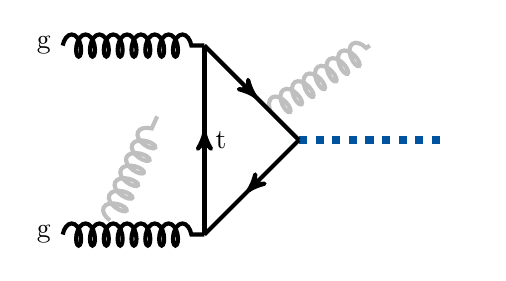
\begin{tikzpicture}[line width=1.5pt, scale=1.2]
\draw[step=0.5cm, very thin, transparent] (0cm,0cm) grid (4cm,2cm);

\draw[gluon, lightgray] (0.5cm,0cm+0.15cm) -- (1cm,1.25cm);
\draw[gluon, lightgray] (1.5cm+0.7cm,1cm+1cm-0.7cm) -- (3.25cm,2cm);

\draw[gluon] (0cm,0cm) -- (1.5cm,0cm);
\node at (0cm-0.2cm,0cm) {g};

\draw[gluon] (0cm,2cm) -- (1.5cm,2cm);
\node at (0cm-0.2cm,2cm) {g};

\draw[scalarnoarrow, color1, line width=3pt] (2.5cm,1cm) -- (4cm,1cm);
\node at (4cm+0.3cm,1cm) [color1]{\PHiggs};

\draw[fermion] (2.5cm,1cm) -- (1.5cm,0cm);
\draw[fermion] (1.5cm,2cm) -- (2.5cm,1cm);
\draw[fermion] (1.5cm,0cm) -- node[right]{t} (1.5cm,2cm);
\end{tikzpicture}

}
\hspace{0.05\textwidth}
\subfloat[VBF]{ \label{figure_higgs_production_feynman_vector_boson_fusion}
	\centering 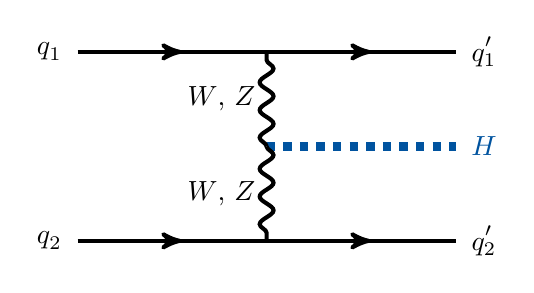
\begin{tikzpicture}[line width=1.5pt, scale=1.2]
\draw[step=0.5cm, very thin, transparent] (0cm,0cm) grid (4cm,2cm);

\draw[fermion] (0cm,0cm) -- (2cm,0cm);
\node at (0cm-0.3cm,0cm) {$q_2$};

\draw[fermion] (2cm,0cm) -- (4cm,0cm);
\node at (4cm+0.3cm,0cm) {$q_2'$};

\draw[fermion] (0cm,2cm) -- (2cm,2cm);
\node at (0cm-0.3cm,2cm) {$q_1$};

\draw[fermion] (2cm,2cm) -- (4cm,2cm);
\node at (4cm+0.3cm,2cm) {$q_1'$};

\draw[scalarnoarrow, color1, line width=3pt] (2cm,1cm) -- (4cm,1cm);
\node at (4cm+0.3cm,1cm) [color1]{$H$};

\draw[vector] (2cm,1cm) -- node[left]{$W$, $Z$} (2cm,0cm);
\draw[vector] (2cm,1cm) -- node[left]{$W$, $Z$} (2cm,2cm);
\end{tikzpicture}

}
\\ \vspace{5mm}
\subfloat[VH]{ \label{figure_higgs_production_feynman_higgs_strahlung}
	\centering 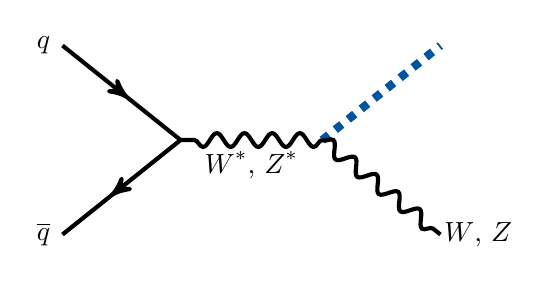
\begin{tikzpicture}[line width=1.5pt, scale=1.2]
\draw[step=0.5cm, very thin, transparent] (0cm,0cm) grid (4cm,2cm);

\draw[fermionbar] (0cm,0cm) -- (1.25cm,1cm);
\node at (0cm-0.2cm,0cm) {$\overline{q}$};

\draw[fermion] (0cm,2cm) -- (1.25cm,1cm);
\node at (0cm-0.2cm,2cm) {$q$};

\draw[scalarnoarrow, color1, line width=3pt] (2.75cm,1cm) -- (4cm,2cm);
\node at (4cm+0.3cm,2cm) [color1]{\PHiggs};

\draw[vector] (2.75cm,1cm) -- node[below]{$W^*$, $Z^*$} (1.25cm,1cm);

\draw[vector] (2.75cm,1cm) -- (4cm,0cm);
\node at (4cm+0.4cm,0cm) {$W$, $Z$};
\end{tikzpicture}

}
\hspace{0.05\textwidth}
\subfloat[ttH]{ \label{figure_higgs_production_feynman_associated_production}
	\centering 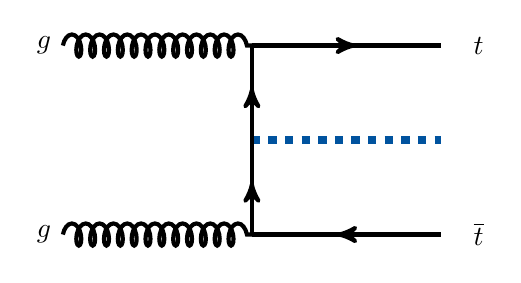
\begin{tikzpicture}[line width=1.5pt, scale=1.2]
\draw[step=0.5cm, very thin, transparent] (0cm,0cm) grid (4cm,2cm);

\draw[gluon] (0cm,0cm) -- (2cm,0cm);
\node at (0cm-0.2cm,0cm) {$g$};

\draw[gluon] (0cm,2cm) -- (2cm,2cm);
\node at (0cm-0.2cm,2cm) {$g$};

\draw[scalarnoarrow, color1, line width=3pt] (2cm,1cm) -- (4cm,1cm);
\node at (4cm+0.3cm,1cm) [color1]{\PHiggs};

\draw[fermion] (4cm,0cm) -- (2cm,0cm);
\node at (4cm+0.4cm,0cm) {$\overline{t}$};

\draw[fermion] (2cm,0cm) -- (2cm,1cm);
\draw[fermion] (2cm,1cm) -- (2cm,2cm);

\draw[fermion] (2cm,2cm) -- (4cm,2cm);
\node at (4cm+0.4cm,2cm) {$t$};
\end{tikzpicture}

}
\caption{Feynman diagrams of the four main Higgs production modes at \LHC.}
\label{figure_higgs_production_feynman}
\end{figure}

The gluon fusion process (ggF)~\ref{figure_higgs_production_feynman_gluon_fusion} is the most dominant production process at \LHC. Two gluons produce a top loop,
which couples to the Higgs boson. The loop can be produced by any quark, but it was shown before, that the fermion mass
is proportional to the coupling to the Higgs boson. This makes the heaviest fermion the most probable to participate in this loop:
the top quark. As shown in the feynman diagram jets can be radiated of the gluons or the loop causing a phenomena called
initial state radiation (ISR). The radiation of jets boosts the Higgs boson, which can be exploited in Higgs searches, but also reduces
the cross section of this Higgs production.

The second most prominent process is vector boson fusion (VBF)~\ref{figure_higgs_production_feynman_vector_boson_fusion}.
Two quarks radiate weak gauge bosons, which annihilate and produce a Higgs boson. The two quarks are then scattered into opposite
directions, leading to a very clear detector signature of two forward jets.

The Higgs strahlung process (VH)~\ref{figure_higgs_production_feynman_higgs_strahlung} is suppressed at \LHC since it requires the
annihilation of two quarks. This process would be the most dominant at a proton-antiproton collider, such as \Tevatron at \Fermilab.
The annihilation produces an excited $\PW^*$ or $\PZ^*$ boson, which deexictes by radiating a Higgs boson.

The last remaining process it the top associated Higgs production (ttH)~\ref{figure_higgs_production_feynman_associated_production}.
This process is highly suppressed, since it requires energies to produce two top quarks and a Higgs boson in the final state. It is
neglected in most analysis.

Figure~\ref{figure_higgs_production_cross_sections} shows the cross sections for the different Higgs productions and their total uncertainties
at the \LHC for two different center-of-mass energies as a function of the Higgs boson mass $m_H$.


\begin{figure}[h]
\includegraphics[width=0.48\textwidth]{figures/Higgs_XS_8TeV_lx.pdf}
\hfill
\includegraphics[width=0.48\textwidth]{figures/YRHXS_Summary_fig3}
\caption[Higgs boson production cross sections.]{Predicted Higgs boson production cross sections for center-of-mass energies of $\sqrt s=\unit{8}{\TeV}$~(left) and \unit{14}{\TeV}~(right)~\cite{yellow_report_1, yellow_report_2, yellow_report_3}.}
\label{figure_higgs_production_cross_sections}
\end{figure}

  \chapter{Higgs Searches \label{chapter3_analysis}}

\section{Higgs Discovery}
The experimental verfication of the existance of a Higgs boson and therefore the Higgs mechanism was found by
the two collaborations \CMS and \ATLAS in July 2012. The observation was found with a significance of $5.0\sigma$ ($5.9\sigma$)
at a Higgs boson mass of approximately $m_H=125$ GeV by \CMS (\ATLAS). It was necessary to combine different decay channel to
achieve the observation with the measured \LHC data of Run 1. Outstanding are the two golden channels $\PH \rightarrow \PZ \PZ \rightarrow 4\Plepton$ and
$\PH \rightarrow \Pgamma \Pgamma$, which profit from a high mass resolution and controllable backgrounds. Figure~\ref{figure_higgs_discovery_cms} shows the
discovery plots of both channel of the CMS collaboration.

\begin{figure}[h]
\includegraphics[width=0.48\textwidth]{../plots/HiggsGG_discovery.pdf}
\hfill
\includegraphics[width=0.48\textwidth]{../plots/HiggsZZ_discovery.pdf}
\caption[Higgs boson discovery CMS.]{Higgs boson discoveries in the two golden channels $\PH \rightarrow \Pgamma \Pgamma$ (left) and $\PH \rightarrow \PZ \PZ \rightarrow 4\Plepton$ (right) by \CMS~\cite{HiggsDiscovery_CMS}.}
\label{figure_higgs_discovery_cms}
\end{figure}

Both discovery plots cleary show an excess in the invariant mass distribution at around $m_H=125$ GeV. The left figure
shows the invariant mass of two photons in a range between $100$ GeV and $160$ GeV. The red dotted line shows the background only
prediction (SM without Higgs boson) and the red line the signal plus background prediction (SM with Higgs boson). Also the $1\sigma$ and $2\sigma$
uncertainties are shown in a brazilian band style. The deviation show of the two hypothesis is cleary shown and is not compatible anymore within
the uncertainties of the measured data.

The right figure shows the $\PH \rightarrow \PZ \PZ \rightarrow 4\Plepton$ channel. Here one can also see that the background only prediction can not
explain any longer the measured data. The signal prediction of a Higgs boson with $m_H=125$ is shown again in red and explains the excess in data very well.
As a small example the basic analysis strategy is depicted in the following section~\ref{golden_channel}.

Both decay channel leave a clear signature in the detecor, which makes the reconstruction of the Higgs boson easier than in most other
channel. Figure~\ref{figure_higgs_discovery_eventdisplay} shows two event displays corresponding to the two discovery plots from figure~\ref{figure_higgs_discovery_cms}.

\begin{figure}[h]
\includegraphics[width=0.48\textwidth]{../plots/cms_event_display.png}
\hfill
\includegraphics[width=0.48\textwidth]{../plots/atlas_event_display.png}
\caption[Higgs boson discovery CMS.]{Higgs boson decay event displays in the two golden channels $\PH \rightarrow \Pgamma \Pgamma$ (left: \CMS) and $\PH \rightarrow \PZ \PZ \rightarrow 4\Plepton$ (right: \ATLAS).}
\label{figure_higgs_discovery_eventdisplay}
\end{figure}

In the left event display~\ref{figure_higgs_discovery_eventdisplay} one can clearly see entries in the electromagnetic calorimeter (ECAL) but not tracks (hinted with the dotted line).
It is the signature of two photons, which interact electromagnetically (entries in ECAL) and have no electrically charge (no tracks). From the event display it is not
possible to reconstruct the invariant mass, therefore it provides only the signatures in the detector for a Higgs boson candidate.

The right event display~\ref{figure_higgs_discovery_eventdisplay} shows four leptons in the detector. Furthermore one can specify them as muons, since they
penetrate the whole detector complex. Unlike photons muons have an electrically charge and therefore leave a track in the inner tracker system of the detector.
This event display also can only show a Higgs boson candidate, since the essential invariant mass information is missing.

In order to prove the observation of the Higgs boson statistical methods are needed. In fact it is a common strategy to perform
hypothesis testing for the theory with and without the Higgs boson. They allow to quantify the compatability between the SM with a Higgs boson and
without a Higgs boson at a certain confidence level (usually chosen to be $95\%$). Figure~\ref{figure_higgs_discovery_limit} (left) shows the limit for a SM Higgs hypothesis as a function
of different mass hypothesis. A clear excess of the data can be observed in the mass interval of $120$ GeV to $130$ GeV. This means that one can not exclude a Higgs boson with $120 < m_H <130$ GeV
with the measured data of Run 1 from the SM.

\begin{figure}[h]
\includegraphics[width=0.48\textwidth]{../plots/higgs_combined_cls.pdf}
\hfill
\includegraphics[width=0.48\textwidth]{../plots/higgs_p_value.pdf}
\caption[Higgs boson discovery CMS limit.]{Expected and observed limit (left) and local p-value (right) as a function of different mass hypothesis ~\cite{HiggsDiscovery_CMS}.}
\label{figure_higgs_discovery_limit}
\end{figure}

Additionally it is possible to quantify the statistical significance of the measured excess.
The local p-value is calculated as a function of the Higgs boson mass. From figure~\ref{figure_higgs_discovery_limit} (right) it is clear
that the combined observed limit shows an excess of $5.0\sigma$, making it a discovery. At the same time the best fit result for the Higgs mass
can be extracted. It is measured to be:
\begin{itemize}
  \item CMS: $m_H= 125.3 \pm 0.4 \,\text{(stat)} \pm 0.5 \,\text{(sys)}\, \text{GeV}$~\cite{HiggsDiscovery_CMS}
  \item ATLAS: $m_H= 126.0 \pm 0.4 \, \text{(stat)} \pm 0.4 \, \text{(sys)}\, \text{GeV}$~\cite{HiggsDiscovery_ATLAS}
\end{itemize}


\begin{figure}[h]
\includegraphics[width=0.75\textwidth]{../plots/higgs_pvalue_table.pdf}
\caption[Higgs boson discovery CMS limit.]{Table of expected and observed statistical significances for different decay channel~\cite{HiggsDiscovery_CMS}.}
\label{figure_higgs_discovery_pvalue}
\end{figure}

The expected and observed significance for all analysed decay channels is depicted in table~\ref{figure_higgs_discovery_pvalue}. It can be seen that
including the $\PH \rightarrow \Ptau \Ptau$ and $\PH \rightarrow \Pbottom \APbottom$ the observed significance drops again. This was due to a bad statistical
fluctuation in the measurement by \CMS.


\section{Golden Channel: $\PH \rightarrow \PZ \PZ \rightarrow 4\Plepton$ \label{golden_channel}}

Although branching fraction of the $\PH \rightarrow \PZ \PZ \rightarrow 4\Plepton$ is quite small ($\approx2.6\%$) it provides a very high
mass resolution and a straight forward reconstruction of the Higgs boson. The basic analysis strategy is to start with the four leptons, which
are measured in the detector, and then reconstruct the $\PZ$ bosons. Afterwards the two $\PZ$ bosons can be combined to the Higgs boson.

As aforementioned one can only start this analysis by selecting four leptons. The possible combinations in this case are: $4\Pe$, $4\Pmu$ or $2\Pe2\Pmu$.
The tau leptons are neglected here, since their reconstruction efficiency is quite small in comparision to muons and electrons. The selection of the
four leptons is done by introducing basic requirements. These cuts reject pile-up events (remnants from pp collisions), which one can see in the event displays from figure~\ref{figure_higgs_discovery_eventdisplay}
as the yellow tracks.

Afterwards it is necessary to reconstruct $\PZ$ boson candidates from the lepton selection. Two opposite sign same flavour leptons are combined. Their resulting invariant
mass has to pass a mass window cut of $12 < m_{ll} < 120$ GeV. One of the combination is required to have the mass of the $\PZ$ mass, since one $\PZ$ boson is produced on-shell: $m_{ll}\approx m_{\PZ}$. The remaining
two leptons are combined to a off-shell $\PZ^*$ boson. For each event one can now combine the invariant mass of the four leptons of the $\PZ\PZ^*$
selection in order to reconstruct the Higgs boson.

After the introduced event selection, the analysis has some remaining irreducible backgrounds. First of all there is the non-resonant $\PZ\PZ$ and $\PZ\Pgamma^*$ process.
From figure~\ref{figure_higgs_background} it is obvious that they represent the main background of this analysis. The other irreducible background are merged into one background class, the so-called $\PZ + \mathrm{X}$ process.
This process is the combination of the following 5 background contributions: $\PZ+$jets, $\Ptop\APtop+$jets, $\PZ\Pgamma+$jets,
$\PW\PW+$jets and $\PW\PZ+$jets. These processes do not leave four leptons in the detector, but instead the jets are misidentified as leptons by the reconstruction requirements.
The rate of this is rather small, but non-negligible.

\begin{figure}[h!]
\centering
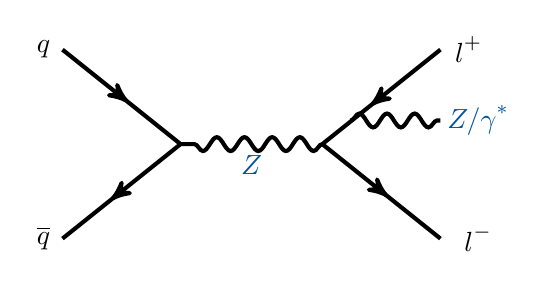
\begin{tikzpicture}[line width=1.5pt, scale=1.2]
\draw[step=0.5cm, very thin, transparent] (0cm,0cm) grid (4cm,2cm);

\draw[fermionbar] (0cm,0cm) -- (1.25cm,1cm);
\node at (0cm-0.2cm,0cm) {$\overline{q}$};

\draw[fermion] (0cm,2cm) -- (1.25cm,1cm);
\node at (0cm-0.2cm,2cm) {$q$};

\draw[fermionbar] (2.75cm,1cm) -- (4cm,2cm);
\node at (4cm+0.3cm,2cm) {$l^+$};

\draw[vector] (2.75cm,1cm) -- node[below]{$\textcolor{color1}{Z}$} (1.25cm,1cm);

\draw[fermion] (2.75cm,1cm) -- (4cm,0cm);
\node at (4cm+0.4cm,0cm) {$l^-$};

\draw[vector] (3.05cm,1.25cm) -- (4cm,1.25cm);
\node at (4cm+0.4cm,1.25cm) {$\textcolor{color1}{Z/\gamma^*}$};
\end{tikzpicture}

\caption{Feynman diagram of the non-resonant background $\PZ\PZ$ and $\PZ\Pgamma^*$ in the $\PH \rightarrow \PZ \PZ \rightarrow 4\Plepton$ analysis.}
\label{figure_higgs_background}
\end{figure}

This analysis was done again with Run 2 data. The Higgs boson was rediscovered, which marks a hugh success. Figure~\ref{figure_higgs_rediscovery_atlas} shows the rediscovery with data of $\luminosity=36.1\fbinv$ taken in year
2016. A brand new (still on-going) analysis is currently at pre-approval. Therefore the signal region is still blinded in figure~\ref{figure_higgs_rediscovery_cms}. Both plots show clearly an observed (expected) excess in data measured
by ATLAS (CMS). Because of a higher integrated luminosity, the increase in center-of-mass energy from Run 1 to Run 2 and the improved analysis strategy, the excess in the four-lepton mass spectrum is larger than before.

\begin{figure}[h]
\includegraphics[width=0.48\textwidth]{../plots/2016_goldenchannel.png}
\caption[Higgs boson rediscovery.]{Higgs rediscovery in golden channel with 2016 data by ATLAS~\cite{HiggsReDiscovery_ATLAS}.}
\label{figure_higgs_rediscovery_atlas}
\end{figure}

\begin{figure}[h]
\includegraphics[width=0.48\textwidth]{../plots/2017_goldenchannel}
\caption[Higgs boson rediscovery.]{Brand new analysis with 2017 data by CMS~\cite{HiggsReDiscovery_CMS} (right, still blinded)}
\label{figure_higgs_rediscovery_cms}
\end{figure}

\section{Recent $\PH \rightarrow \Ptau \Ptau$ Discovery \label{HTT}}

In Run 1 the search for the SM Higgs boson decaying into a pair of tau leptons suffered from bad statistical fluctuations. Additionally this measurement
is very challenging, since the reconstruction efficiency of tau leptons is rather bad in comparison to electrons and muons. Also this search has to deal with
the QCD background, which is very hard to predict and badly modelled by Monte Carlo (MC) simulations.

Recently the decay of the SM Higgs boson into a pair of tau leptons could be observed by \CMS. One of the most important approach in this analysis is to predict the QCD background from an exclusive
region in data (not from MC). Using the ABCD method one is able to construct control regions for this background and therefore constrain
the systematic uncertainty of the QCD cross-section. Additionally the analysis is splitted into different categories in order to enhance the sensitivity: 0-jet, VBF and boosted category.
Figure~\ref{figure_higgs_discovery_HTT} shows the two discovery plots of the
$\PH \rightarrow \Ptau \Ptau$ analysis. One can clearly see and excess in data in the invariant di-tau mass spectrum. This is especially visible in the "integrated" figure, where
data minus background is shown. The statistical significance of the analysis is measured to be $5.9\sigma$, making it a discovery. The best fit value for the SM Higgs boson
signal strength is $\mu = 1.09_{-0.26}^{+0.27}$ at a Higgs boson mass of $m_{H} = 125.09$ GeV.

\begin{figure}[h]
\includegraphics[width=0.48\textwidth]{../plots/higgstautau_otherchannel.png}
\hfill
\includegraphics[width=0.48\textwidth]{../plots/higgstautau.png}
\caption[Higgs boson discovery $\PH \rightarrow \Ptau \Ptau$.]{Discovery plots of a SM Higgs boson decaying into a pair of tau leptons. Left: Semi-leptonic decay channels. Right: Full-hadronic decaychannel.~\cite{HTT_discovery}.}
\label{figure_higgs_discovery_HTT}
\end{figure}

  \chapter{Conclusion \label{chapter4_conclusion}}


\section{Measurements of the Properties of the Higgs Boson}

The collaborations \CMS and \ATLAS combined their measurements after Run 1 in order to measure the Higgs mass and
the coupling to fermions with higher precision.

The combination of the Higgs mass was measured in the $\PH \rightarrow \PZ \PZ \rightarrow 4\Plepton$ and
$\PH \rightarrow \Pgamma \Pgamma$ channel. A likelihood fit was performed in order to extract the best fit result for
$m_H$ from data. Figure~\ref{figure_higgs_mass} shows the likelihood parabola, where the minimum depicts the best fit value for $m_H$. Furthermore
one can directly extract the $1\sigma$ ($2\sigma$) uncertainty from this plot by looking at the value for $m_H$ for $-2\mathrm{ln} \Lambda(m_H)=1 \,(4)$.
The best fit value for the Higgs mass was determined to be:
$m_H=125.09 \pm 0.21 \text{(stat.)} \pm 0.11 \text{(syst.)}$ GeV.

\begin{figure}[h]
\includegraphics[width=0.75\textwidth]{../plots/higgsmass}
\caption[Higgs boson mass.]{Combined likelihood fit of the Higgs boson mass by \ATLAS and \CMS~\cite{HiggsMass}.}
\label{figure_higgs_mass}
\end{figure}

As aforementioned the Higgs coupling was measured in a combined measurement. The coupling strength of the Higgs boson was predicted
to be proportional to the mass of the fermions or vector bosons. It is shown in figure~\ref{figure_higgs_coupling}, that this predictions holds
within the uncertainties of the data points. A deviation in data from this fit would already be a clear hint to something new. Therefore it is necessary to study
all the SM Higgs boson decays with a very high precision.

\begin{figure}[h]
\includegraphics[width=0.75\textwidth]{../plots/higgscoupling_masses}
\caption[Higgs boson coupling.]{Higgs coupling to fermions or vector bosons as a function of the particle massesn by \ATLAS and \CMS~\cite{HiggsMass}.}
\label{figure_higgs_coupling}
\end{figure}

By measuring the SM Higgs decaying into a pair of photons and a pair of tau leptons it is directly clear that the measured Higgs boson is a spin-0 particle and
electrically neutral. Unfortunately the amount of data is still too low to measure the CP eigenvalue of the Higgs boson. The SM Higgs is predicted to have a
CP eigenvalue of +1. A deviation of this value in a measurement would directly point to physics beyond the SM (BSM).

\section{Exciting Times Ahead...}

With the observation of a new scalar boson in July 2012 a milestone in particle physics was set. Now it is essential to measure all the properties
of the Higgs boson with very high precision. Furthermore the Higgs boson can be used as a probe for new physics. Searches for dark matter produced in
association with a Higgs boson are already ongoing. It is still not clear if there is only one Higgs boson or even more. Many BSM theories (like supersymmetry) require two Higgs doublets, which
predict in total 5 Higgs bosons. Obviously these discoveries are only possible with upgrades in the experiments \CMS and \ATLAS and the accelerator \LHC.

At \LHC there is a future plan until 2035 to upgrade the experiment after Run 3 to a high luminosity machine (HL-LHC). The timetable is shown in figure~\ref{figure_hllhc}.

\begin{figure}[h]
\includegraphics[width=0.75\textwidth]{../plots/hllhc.png}
\caption[HL-LHC]{Future plan of \LHC. A high luminosity upgrade is planned after Run3 until 2035~\cite{HL-LHC}.}
\label{figure_hllhc}
\end{figure}

This upgrade will have some consequences. The main consequence is an increase in pile-up events, which makes data reconstructing even harder than before.
Also an increased amount of data is very challenging for the trigger systems and storage systems.

A new experiment is currently planned in Japan, the so-called International Linear Collider (ILC). Its main purpose is to measure
the mass, the interaction strengths and the CP properties of the Higgs boson with a very high precision. An accelerator of this kind is often referred to as
a Higgs-factory.

All of these developments in Higgs physics will keep the future very interesting. New exciting results will definitely pop up in the near future.

  %% To ignore a specific chapter while working on another, making the build faster, comment it out
\end{mainmatter}

% bib

\bibliographystyle{latex/lucas_unsrt}
\bibliography{writeup}
\end{document}
